\documentclass[12pt,a4paper]{article}
\usepackage[utf8]{inputenc}
\usepackage[german]{babel}
\usepackage[T1]{fontenc}
\usepackage{amsmath}
\usepackage{amsfonts}
\usepackage{amssymb}
\usepackage{graphicx}
\usepackage{siunitx}
\usepackage{float}
\usepackage[left=2cm,right=2cm,top=2cm,bottom=2cm]{geometry}
\author{Gerald}

\begin{document}
\sisetup{separate-uncertainty = true}
	\setlength{\parindent}{0pt} 
	\begin{center}
		{\LARGE Versuchsprotokoll}\\
		\begin{large}
			zum Fortgeschrittenenpraktikum im Bachelorstudiengang Physik\\[0.4cm]
			an der RWTH Aachen\\
			II. Physikalisches Institut A\\[5.5cm]
			\Large\textbf{\textsl{Mößbauerspektroskopie (T05)}}\\[5.5cm]
			\normalsize\textit{vorgelegt\\von}\\[0.4cm]
			\large{Moritz Berger (355244)\\Gerald Kolter (355005)}\\\textbf{Gruppe 30}\\[2cm]
			\large \textbf{Wintersemester 2017/18}
		\end{large}
	\end{center}
	\newpage
	
	\tableofcontents
	\newpage

\section{Versuchsziel}
Das Ziel des Versuchs besteht darin, mithilfe der Mößbauerlinie folgende quantenmechanische Energieaufspaltungen von Eisen zu vermessen:
\begin{enumerate}
\item Die magnetische Hyperfeinstruktur
\item die elektrische Quadrupolaufspaltung
\end{enumerate}
Zudem soll das Einlinienspektrum von Eisen aufgenommen und der Extinktionswirkungsquerschnitt von Eisen, Stahl und Eisensulfat vermessen werden.

\section{Aufbau}
Der Aufbau zur Mößbauerspektroskopie besteht aus einer von einem Transducer in Strahlrichtung bewegten $^{57}$Co Quelle, einem Absorber und einem Detektor. Die Quelle sendet $\gamma$-Strahlung verschiedener Energie aus, wobei hauptsächlich die \SI{14,4}{keV} Linie betrachtet wird. Der Detektor zählt einzelne $\gamma$-Quanten innerhalb eines Energieintervalls, wobei 1024 Kanäle zur Verfügung stehen. Der Transducer bewegt die Quelle sinusförmig.

\section{Durchführung}

\begin{table}
\centering
\begin{tabular}{|c|c|}
\hline 
Spannung am Proportionalzählrohr & \SI{2}{kV} \\ 
\hline 
Messmodus & Pulshöhenanalyse (PHA-Modus) \\
\hline 
Messbereich im PHA-Modus & \SI{4,2}{V} - \SI{6,4}{V} \\
\hline 
\end{tabular} 
\caption{Allgemeine Messeinstellungen.}
\label{tab:Mess_Einstellungen}
\end{table}

Tabelle \ref{tab:Mess_Einstellungen} zeigt die verwendeten Messeinstellungen. Um bei für jede Messung den relevanten Energiebereich vermessen zu können, wurde die Transducer-Geschwindigkeit verändert. Die aus aus der Bewegung resultierende Dopplerverschiebung  ergibt eine Energieverschiebung, mit der die zu messenden Aufspaltungen aufgenommen werden können.

\subsection{Kalibration}
Da der Detektor die gemessenen Zählraten in der Energie auf 1024 Kanäle aufteilt, muss eine Kalibration dieser Kanäle auf die Energie erfolgen. Dazu wird die Geschwindigkeit der Bewegung der Quelle mit einem Michelson-Interferometer gemessen und daraus über den Dopplereffekt die Energie der so verschobenen Linie berechnet. Diese Messungen wurden als Einzige mit dem Multi-Chanel-Scaler-Modus (MCS-Modus) aufgenommen. Diese Messung muss für jede neu eingestellte Transducer-Geschwindigkeit wiederholt werden.

\subsection{Rauschmessung}
Um auf eine mögliche Nullrate korrigieren zu können, wird eine Messung ohne Quelle und ohne Absorber (mit leerem Absorberhalter) aufgenommen.

\subsection{Quellenspektrum}
Für die Mößbauerspektroskopie muss zunächst die Mößbauerlinie gesucht werden. Dazu wird das gesamte Spektrum einmal mit und einmal ohne Bewegung der Quelle aufgenommen. Für die Aufnahme des gesamten Quellspektrums wurde der Messbereich des PHA-Modus auf den maximal einstellbaren Bereich von \SI{10}{mv} - \SI{10}{V}.

\subsection{Extinktionswirkungsquerschnitt}
Zur Bestimmung des Extinktionswirkungsquerschnitts $D_{ex}$ wird das Spektrum insgesamt vier mal aufgenommen:
\begin{enumerate}
\item Mit einem Stahl-Absorber
\item mit einem reinen Eisen-Absorber
\item mit einem FeSO$_4$ $\cdot$ 7H$_2$O-Absorber
\item ohne Absorber 
\end{enumerate} 
Der Extinktionswirkungsquerschnitt kann dann gemäß
\begin{equation}
D_{ex} = R(v) \cdot \dfrac{Z(v = \infty)}{Z(v)} = \dfrac{Z(v = \infty)}{Z(ohne Absorber)}
\end{equation}
bestimmt werden, wobei Z die gesamte Zählrate ist. Für $v = \infty$ ist in der Realität eine Geschwindigkeit von wenigen mm/s ausreichend.

\subsection{Einlinienspektrum}
Das Einlinienspektrum wurde mit einem Absorber aus Stahl aufgenommen.

\subsection{Magnetische Hyperfeinstrukturaufspaltung}
Für die Vermessung der magnetischen Hyperfeinstrukturaufspaltung wurde das Spektrum mit einem Absorber aus reinem Eisen aufgenommen.

\subsection{Elektrische Quadrupolaufspaltung}
Für die Vermessung der elektrischen Quadrupolaufspaltung wird ein FeSO$_4$ $\cdot$ 7H$_2$O-Absorber verwendet. Hier ist im Gegensatz zu den anderen Messungen nur der Linienabstand und nicht die Linienform entscheidend.

\section{Ergebnisse}
\subsection{Kalibration}

\subsection{Rauschmessung}
\subsection{Quellenspektrum}
\subsection{Extinktionswirkungsquerschnitt}

\subsection{Einlinienspektrum}
\begin{figure}
\centering
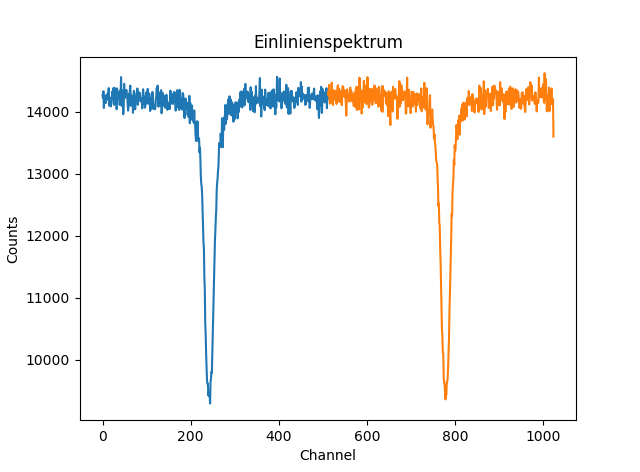
\includegraphics[scale=0.8]{Bilder/Einlinien/Ein_Rohdaten.png}
\caption{Messrate aufgetragen gegen den Channel.}
\label{fig:Ein_Roh}
\end{figure}

In Abbildung \ref{fig:Ein_Roh} sind die Rohdaten der Vermessung des Einlinienspektrums dargestellt.\\


\subsection{Magnetische Hyperfeinstrukturaufspaltung}
\subsection{Elektrische Quadrupolaufspaltung}

\section{Fazit}


\newpage
\section{Anhang}
\subsection{Kalibration}
\begin{figure} [H]
\centering
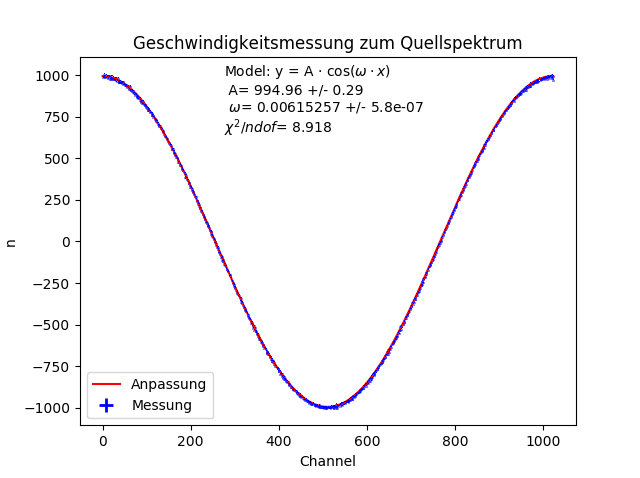
\includegraphics[scale=0.8]{Bilder/Kalibration/Quellspektrum.png}
\caption{Aufnahme zur Geschwindigkeits- und Energiekalibration vor der Messung des Quellspektrums.}
\end{figure}

\begin{figure} [H]
\centering
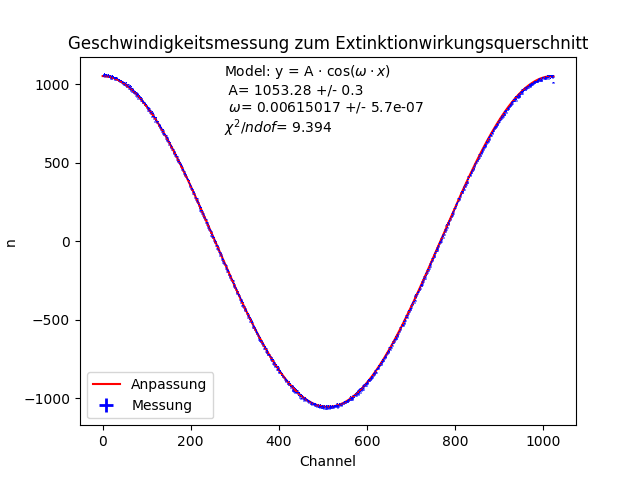
\includegraphics[scale=0.8]{Bilder/Kalibration/Extinktion.png}
\caption{Aufnahme zur Geschwindigkeits- und Energiekalibration vor der Messung des Extinktionswirkungsquerschnitts.}
\end{figure}

\begin{figure} [H]
\centering
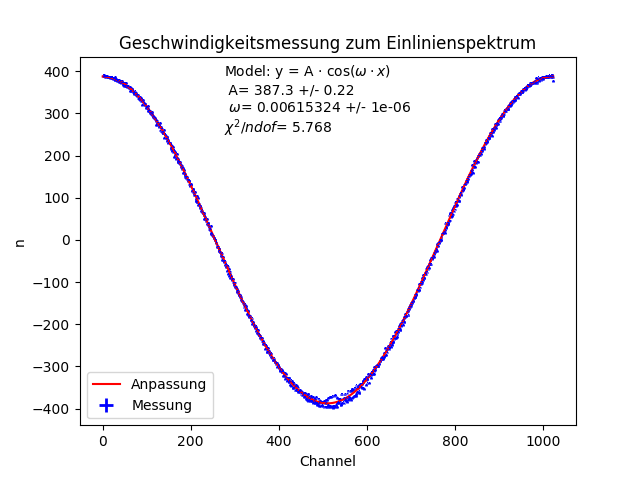
\includegraphics[scale=0.8]{Bilder/Kalibration/Einlinien.png}
\caption{Aufnahme zur Geschwindigkeits- und Energiekalibration vor der Messung des Einlinienspektrums.}
\end{figure}

\begin{figure} [H]
\centering
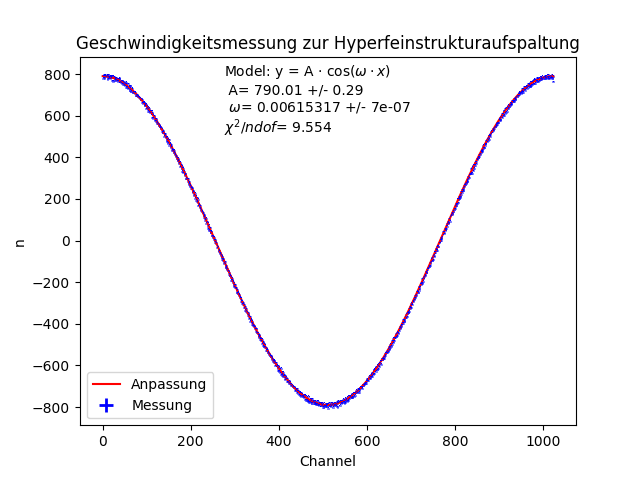
\includegraphics[scale=0.8]{Bilder/Kalibration/Hyperfein.png}
\caption{Aufnahme zur Geschwindigkeits- und Energiekalibration vor der Messung der magnetischen Hyperfeinstrukturaufspaltung.}
\end{figure}

\begin{figure} [H]
\centering
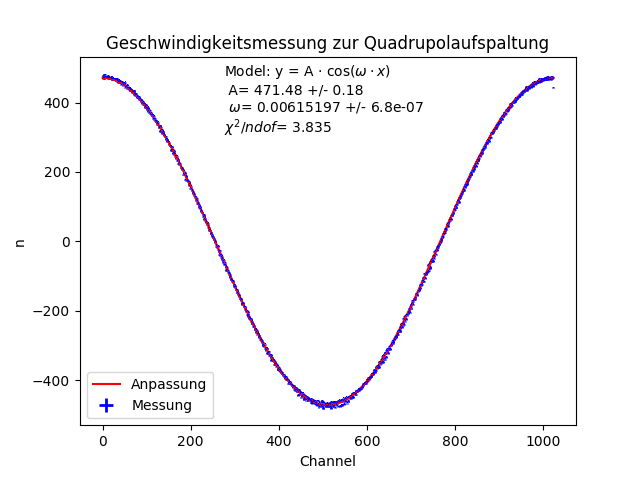
\includegraphics[scale=0.8]{Bilder/Kalibration/Quadrupol.png}
\caption{Aufnahme zur Geschwindigkeits- und Energiekalibration vor der Messung der elektrischen Quadrupolaufspaltung.}
\end{figure}

\subsection{Quellenspektrum}
\subsection{Extinktionswirkungsquerschnitt}
\subsection{Einlinienspektrum}
\subsection{Magnetische Hyperfeinstrukturaufspaltung}
\subsection{Elektrische Quadrupolaufspaltung}


\end{document}
